\chapter*{De Gujō à Kyoto\markboth{De Gujō à Kyoto}{}}
\section*{24 août 2015}
\`A une journée de vélo de Gujō j'arrive à Kakamigahara. Je reste une semaine en wwoofing chez Xavier et Yuka, un couple belge/japonais. 
\begin{center} 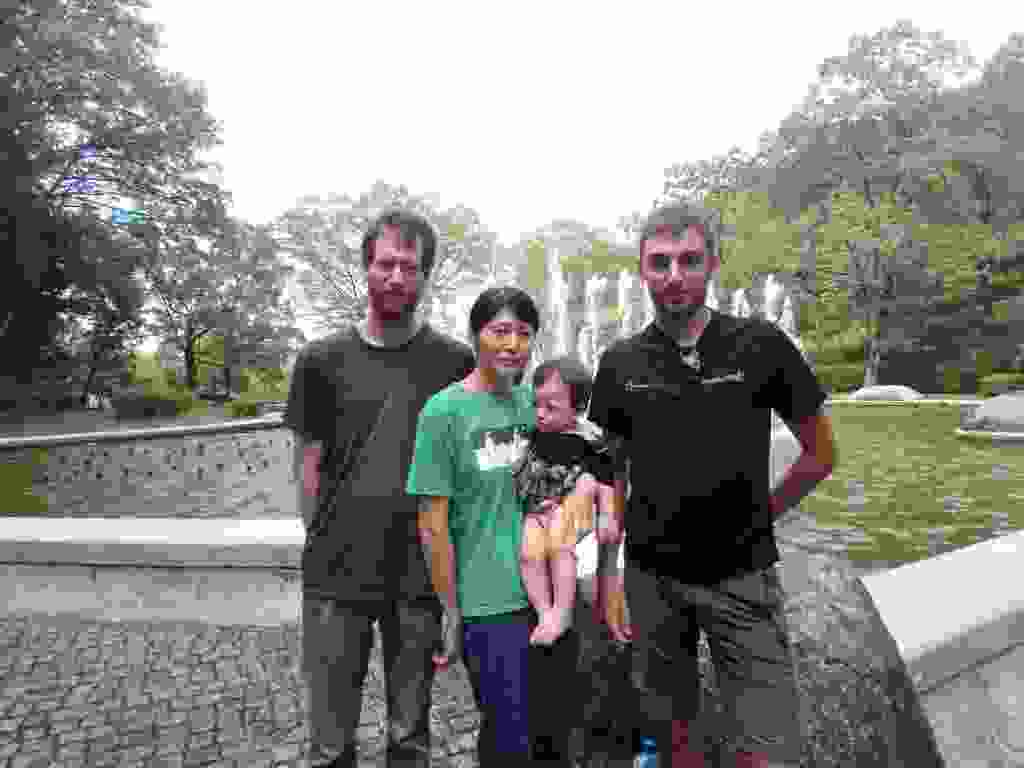
\includegraphics[width=\mywidth]{../wp-content/uploads/2015/08/P8166185-1024x768.jpg} \end{center}

 Le principe du wwoofing est d'aider dans une ferme en échange du gîte et du couvert. 

\pagebreak
 Xavier a plusieurs rizières et un champ en maraîchage. Il expérimente les principes de l'agriculture naturelle, technique issue du Japon. 
\begin{center} 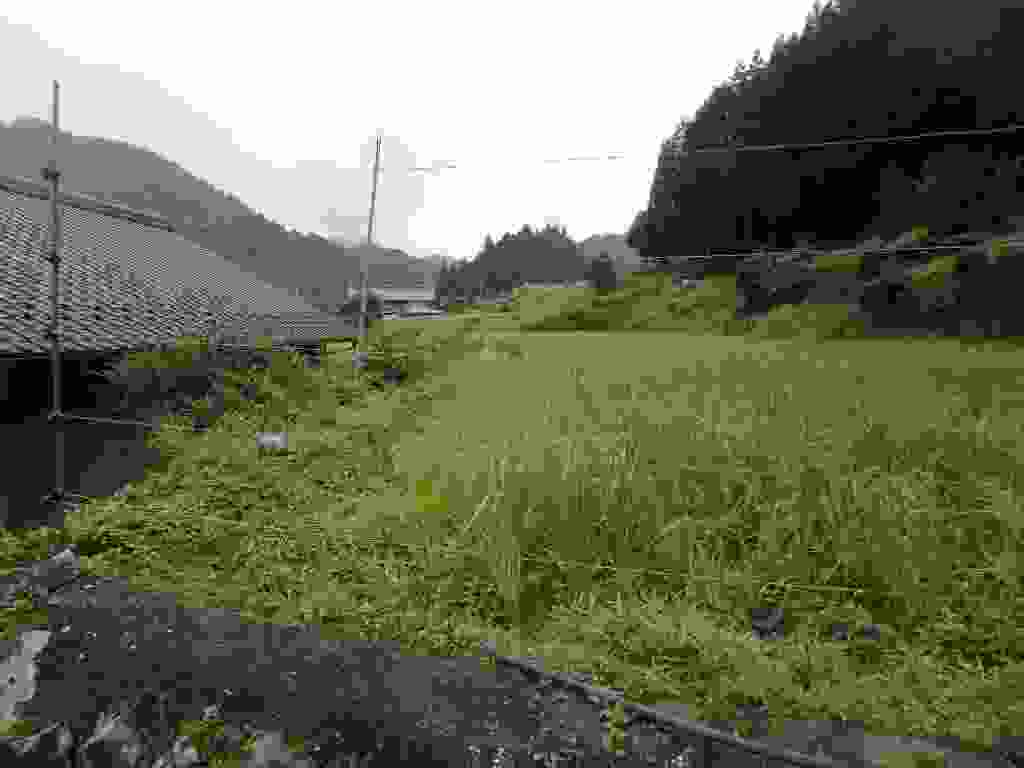
\includegraphics[width=\mywidth]{../wp-content/uploads/2015/08/P8146136-1024x768.jpg} \end{center}
\begin{center} 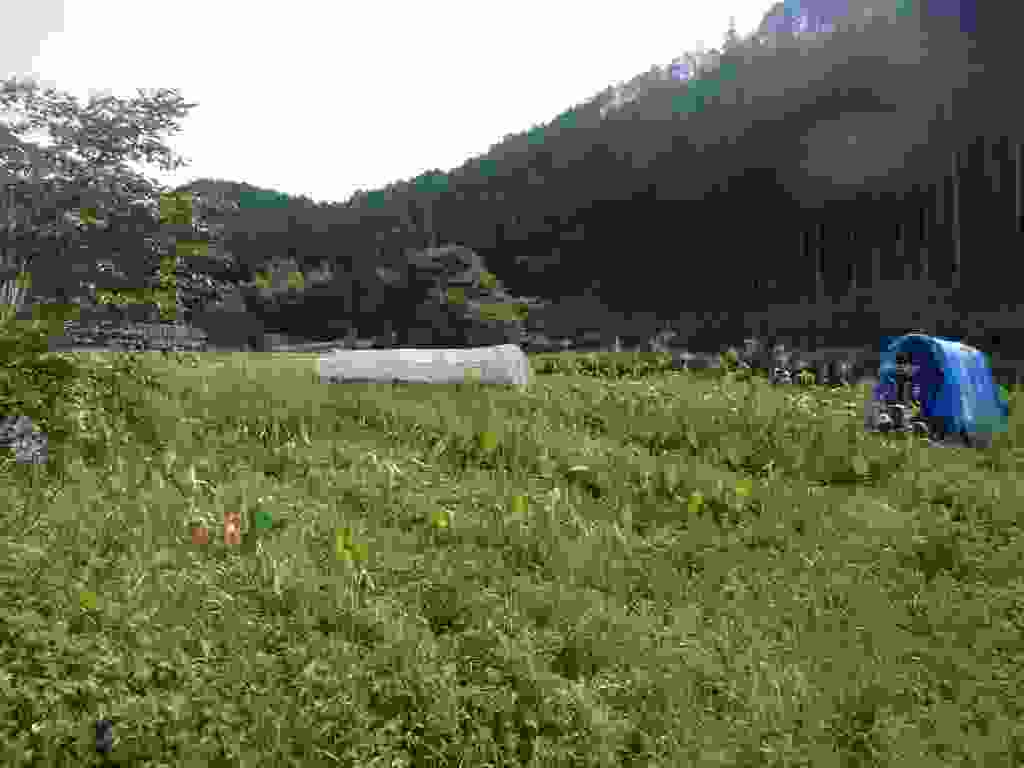
\includegraphics[width=\mywidth]{../wp-content/uploads/2015/08/P8116128-1024x768.jpg} \end{center}

\pagebreak
 Kakamigahara est le centre de l'aéronautique au Japon, un musée y est consacré. 
\begin{center} 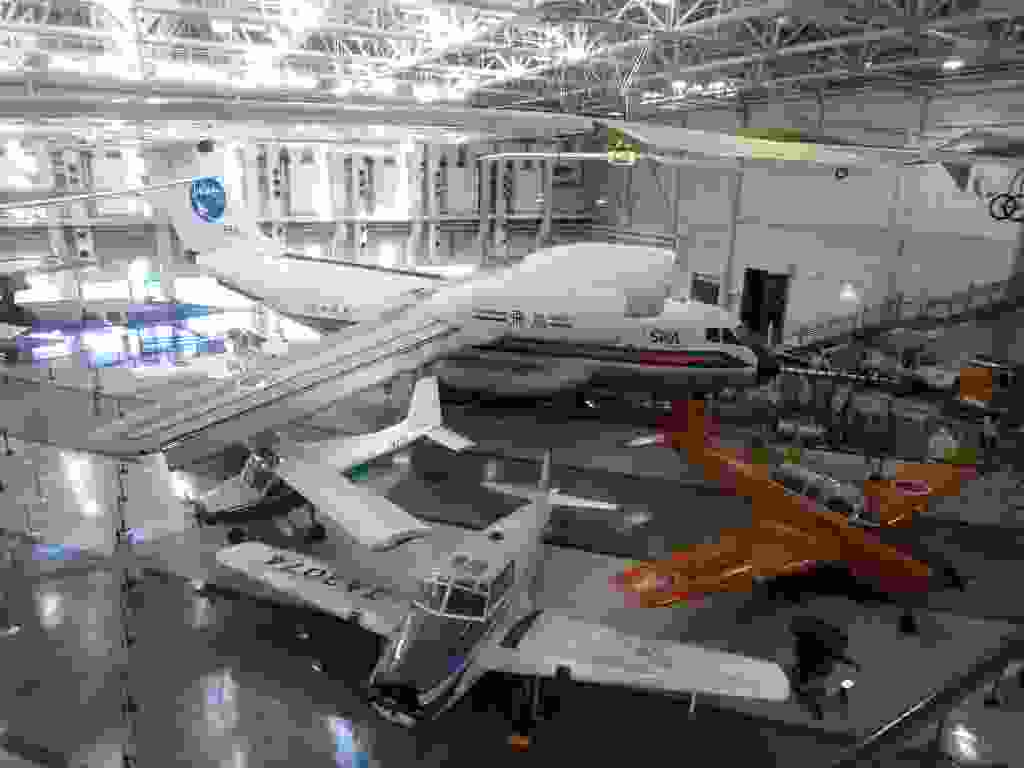
\includegraphics[width=\mywidth]{../wp-content/uploads/2015/08/P8156175-1024x768.jpg} \end{center}
\begin{center} 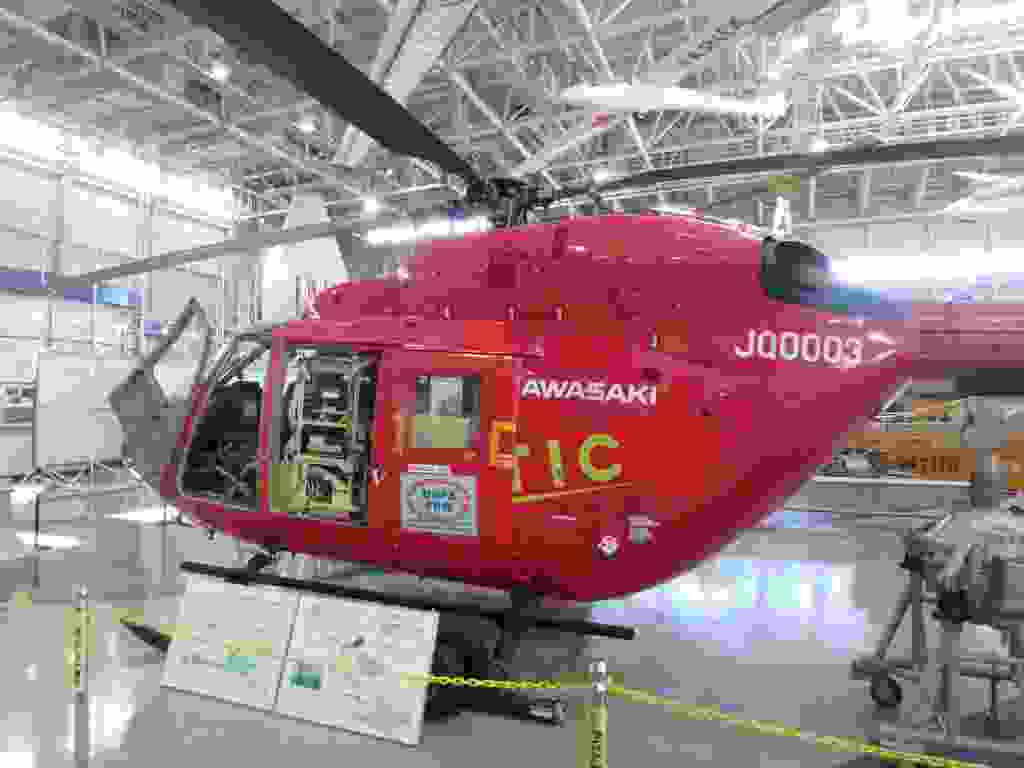
\includegraphics[width=\mywidth]{../wp-content/uploads/2015/08/P8156173-1024x768.jpg} \end{center}

\pagebreak
 \`A coté la ville d'Inuyama : son célèbre château.
\begin{center} 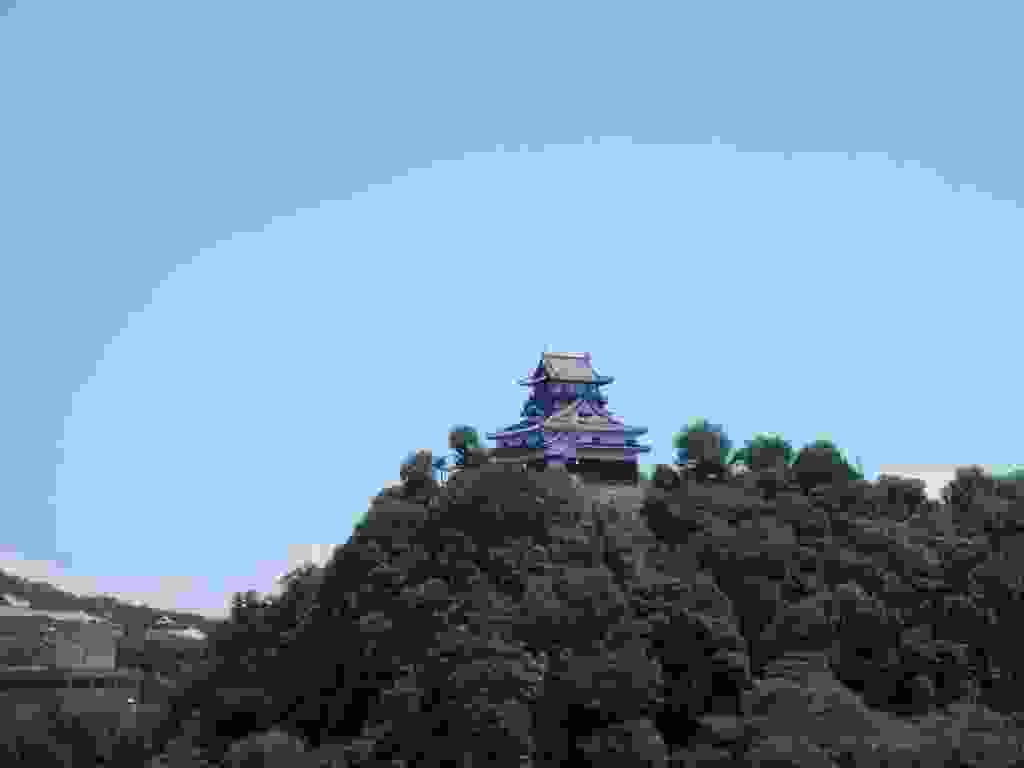
\includegraphics[width=\mywidth]{../wp-content/uploads/2015/08/P8156139-1024x768.jpg} \end{center}
\begin{center} 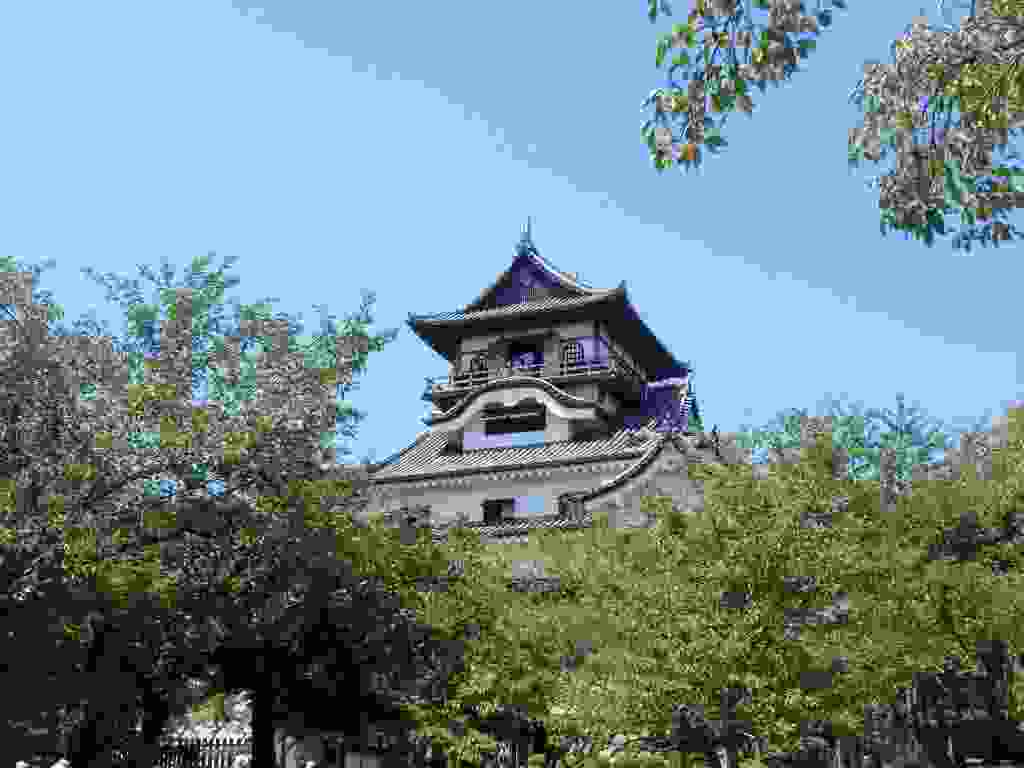
\includegraphics[width=\mywidth]{../wp-content/uploads/2015/08/P8156148-1024x768.jpg} \end{center}

\pagebreak
 Le jardin Jo-an avec des maisons de thé.
\begin{center} 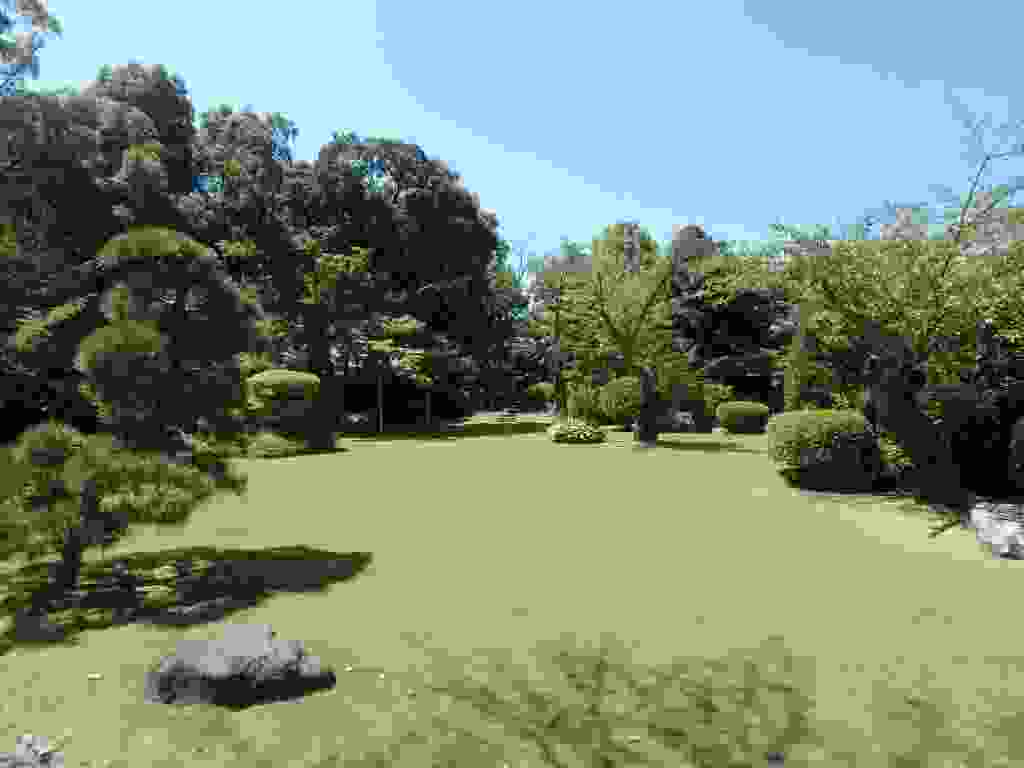
\includegraphics[width=\mywidth]{../wp-content/uploads/2015/08/P8156150-1024x768.jpg} \end{center}
\begin{center} 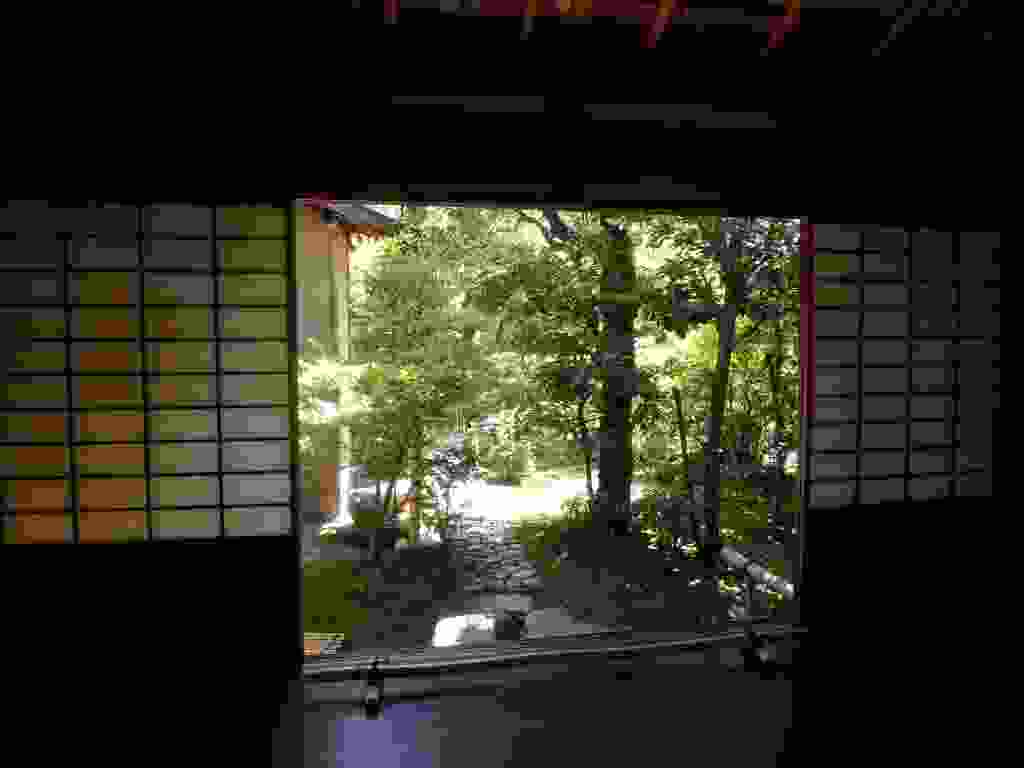
\includegraphics[width=\mywidth]{../wp-content/uploads/2015/08/P8156149-1024x768.jpg} \end{center}
\begin{center} 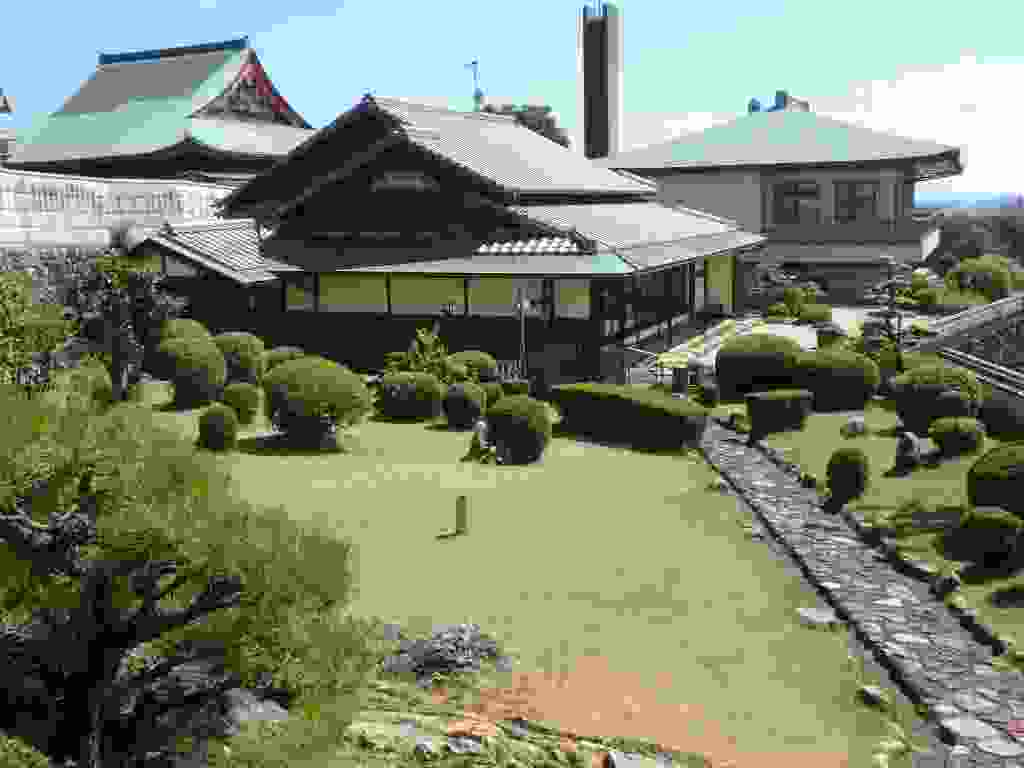
\includegraphics[width=\mywidth]{../wp-content/uploads/2015/08/P8156167-1024x768.jpg} \end{center}

 Le temple de Zuizen-ji.
\begin{center} 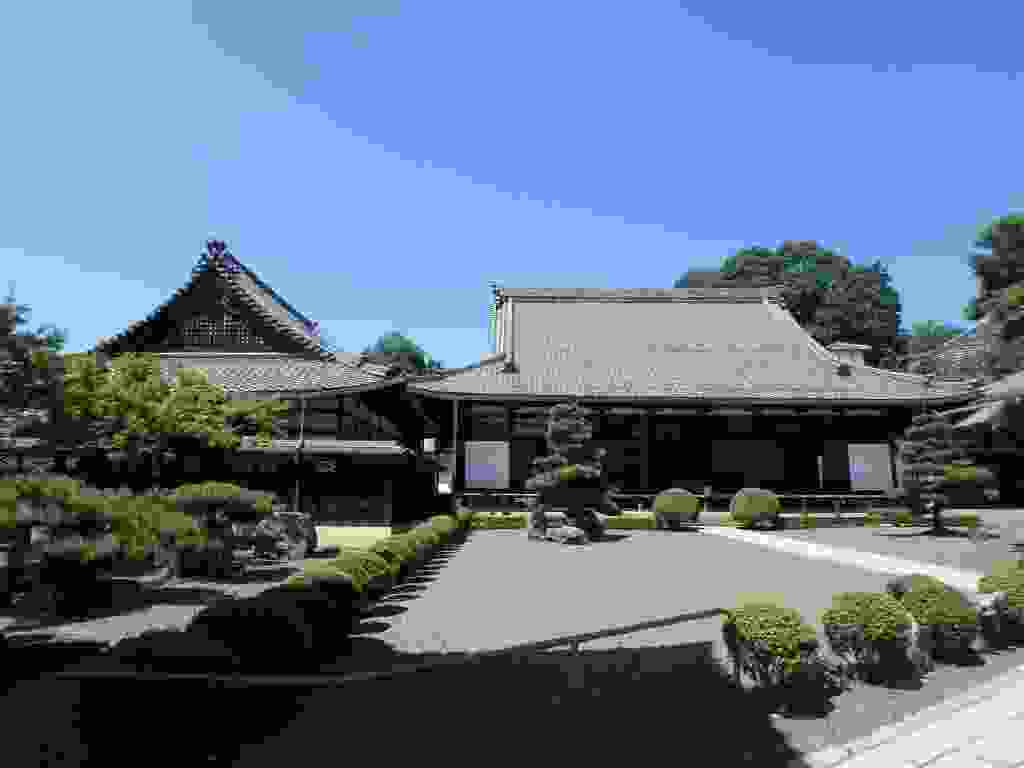
\includegraphics[width=\mywidth]{../wp-content/uploads/2015/08/P8156154-1024x768.jpg} \end{center}

\pagebreak
 \`A Gifu, j'assiste au spectacle nocturne de la pêche aux cormorans. 
\begin{center} 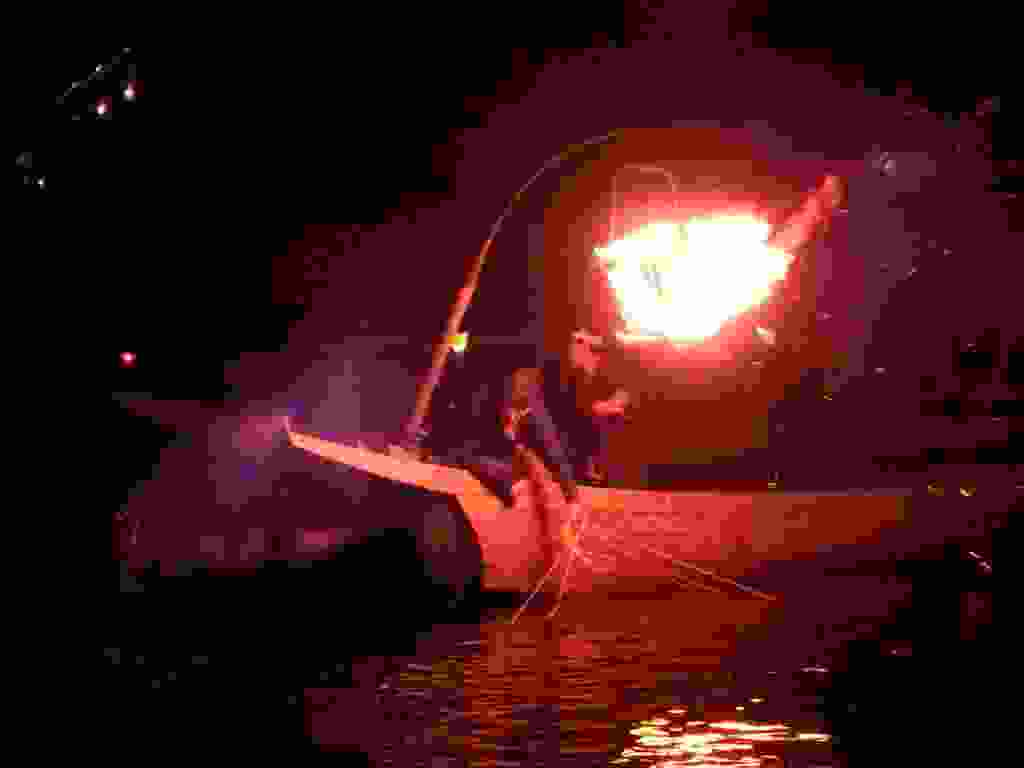
\includegraphics[width=\mywidth]{../wp-content/uploads/2015/08/P8166194-1024x768.jpg} \end{center}
\begin{center} 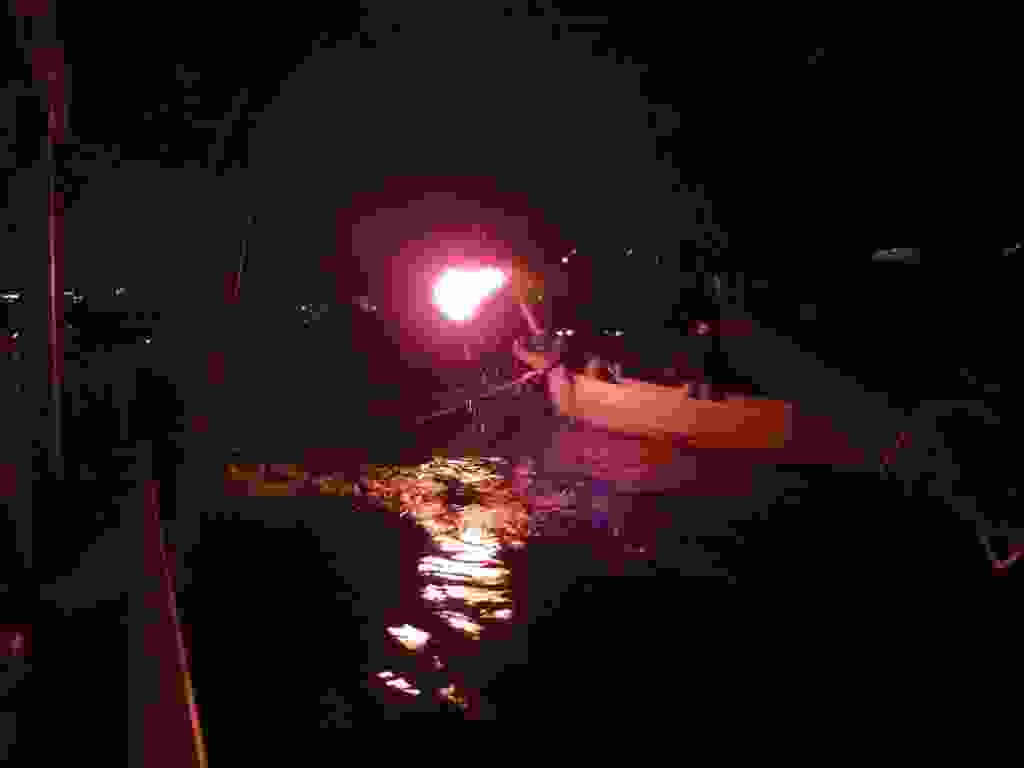
\includegraphics[width=\mywidth]{../wp-content/uploads/2015/08/P8166195-1024x768.jpg} \end{center}
\begin{center} 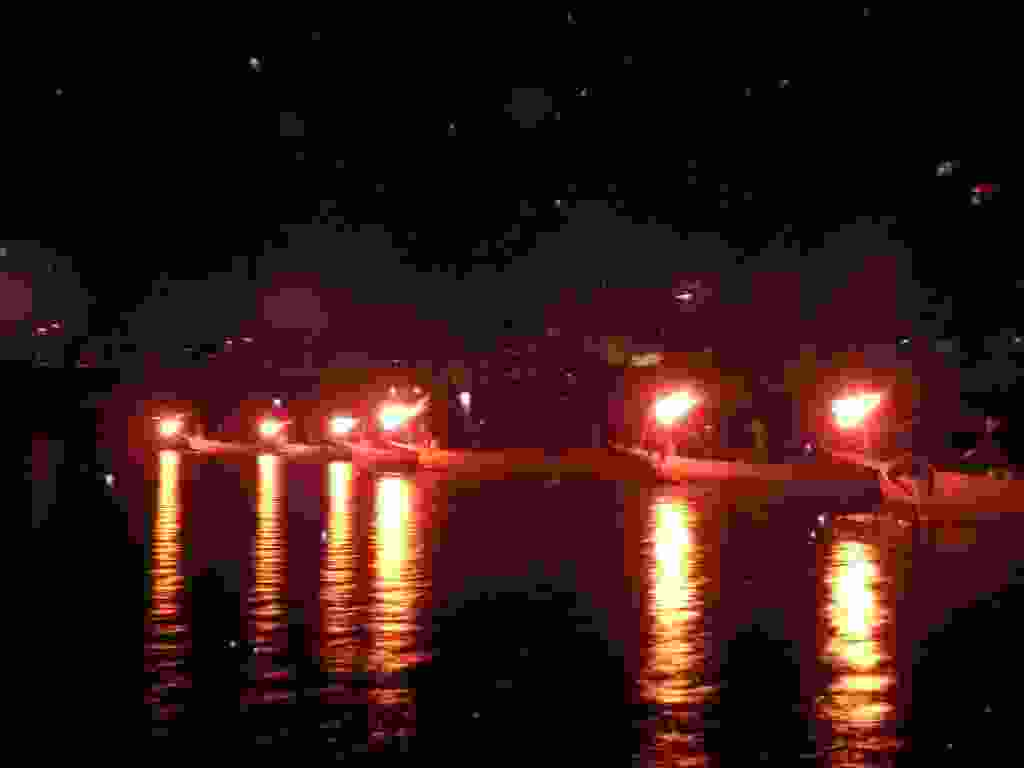
\includegraphics[width=\mywidth]{../wp-content/uploads/2015/08/P8166200-1024x768.jpg} \end{center}

 Je repars en direction de Kyoto et je m'arrête au château d'Hikone.
\begin{center} 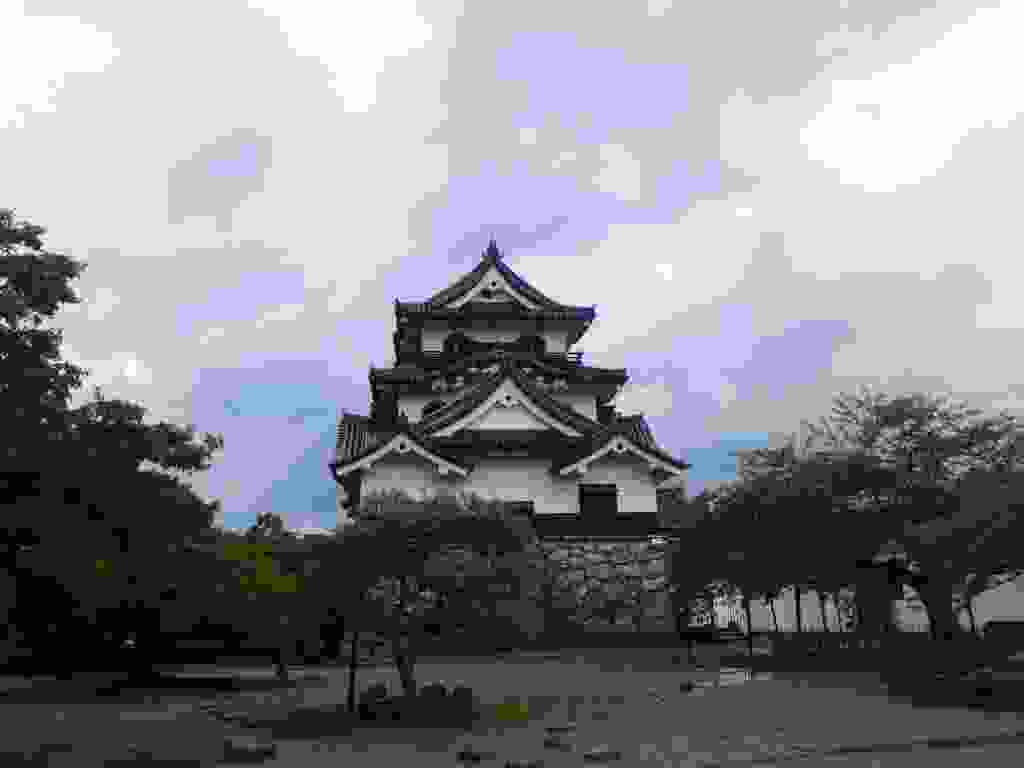
\includegraphics[width=\mywidth]{../wp-content/uploads/2015/08/P8176204-1024x768.jpg} \end{center}

\pagebreak
 Beau jardin en contrebas du château.
\begin{center} 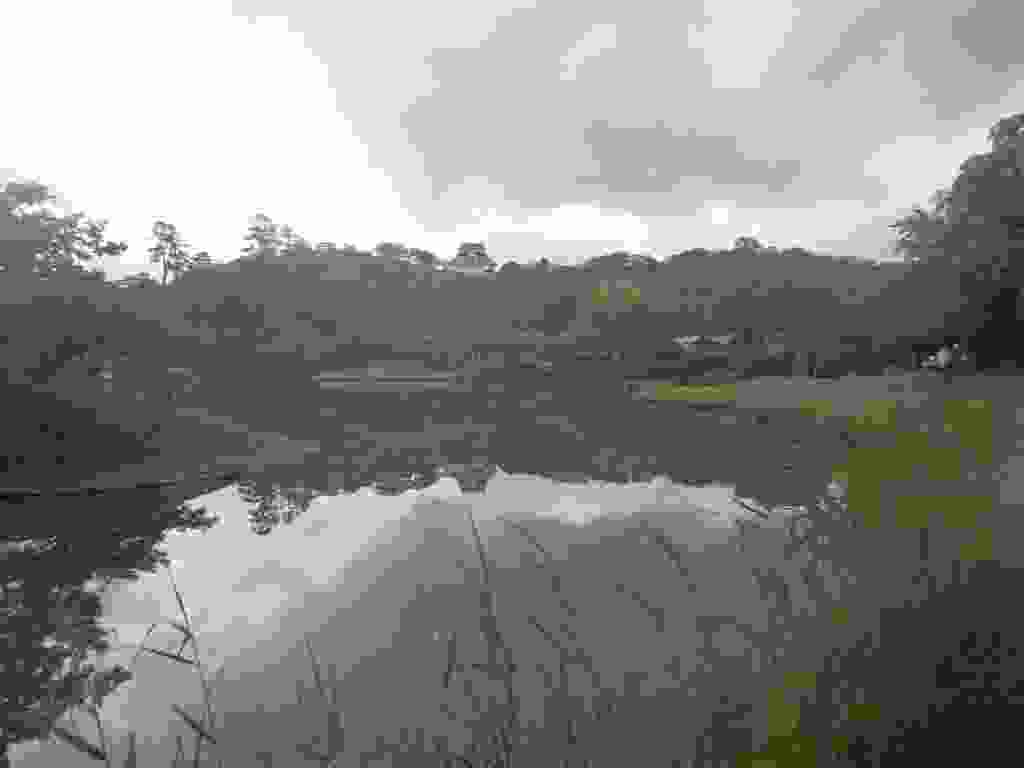
\includegraphics[width=\mywidth]{../wp-content/uploads/2015/08/P8176214-1024x768.jpg} \end{center}
\begin{center} 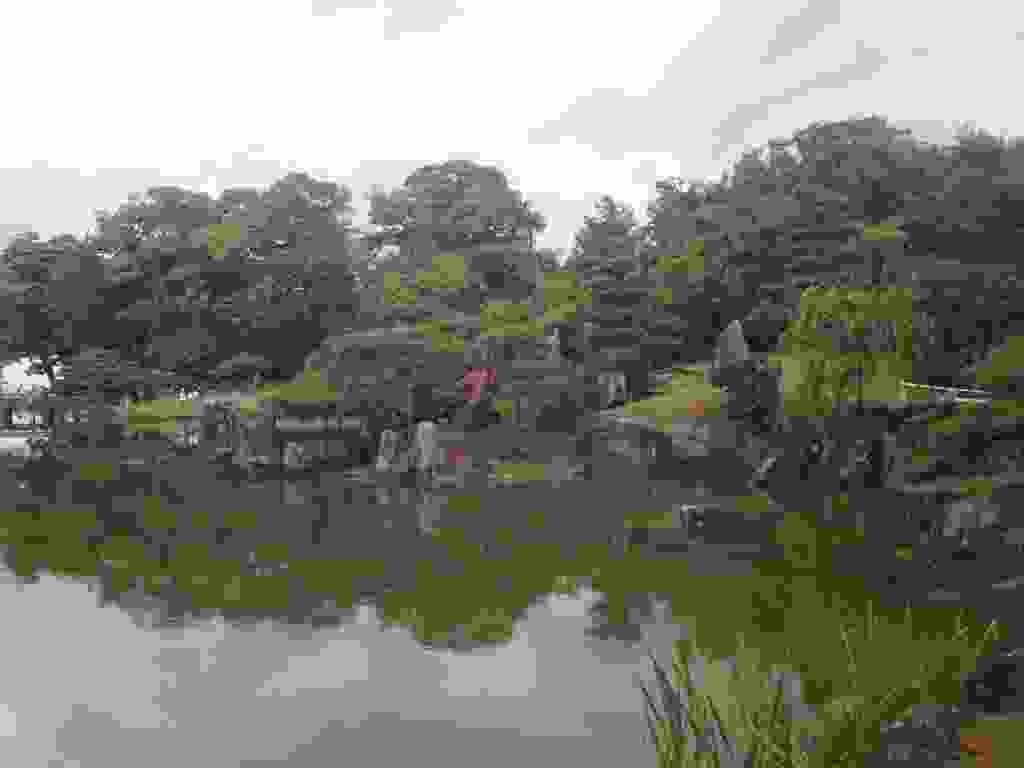
\includegraphics[width=\mywidth]{../wp-content/uploads/2015/08/P8176217-1024x768.jpg} \end{center}

\pagebreak
 Je longe ensuite le lac Biwa, le plus grand du Japon.
\begin{center} 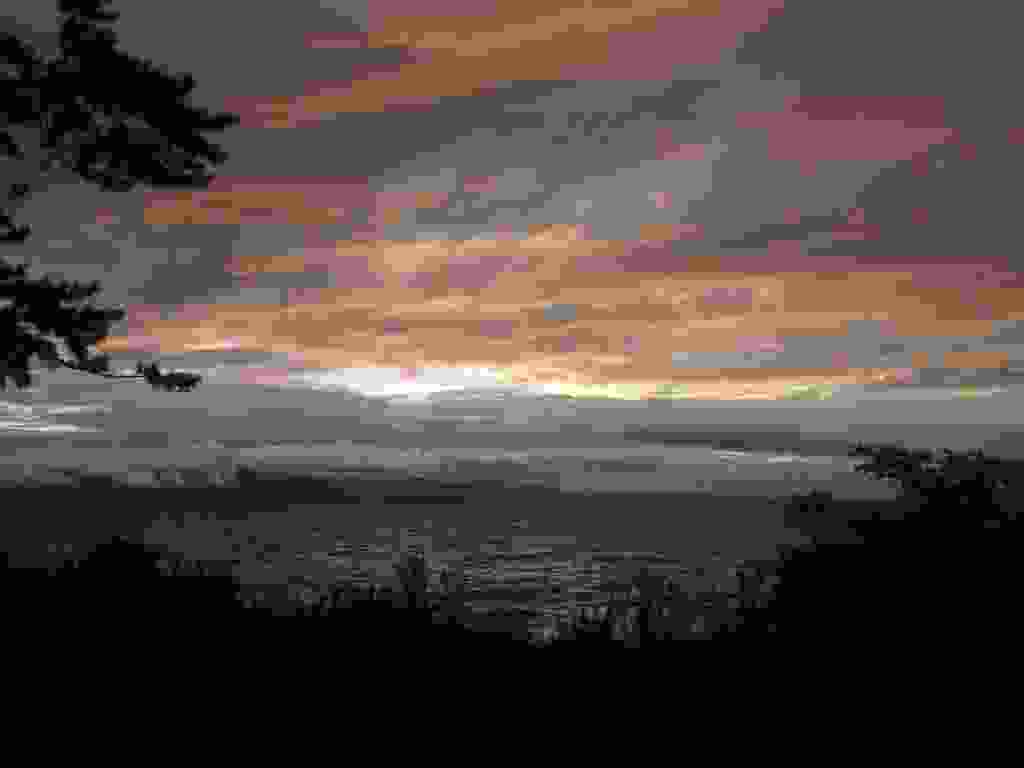
\includegraphics[width=\mywidth]{../wp-content/uploads/2015/08/P8176222-1024x768.jpg} \end{center}
\begin{center} 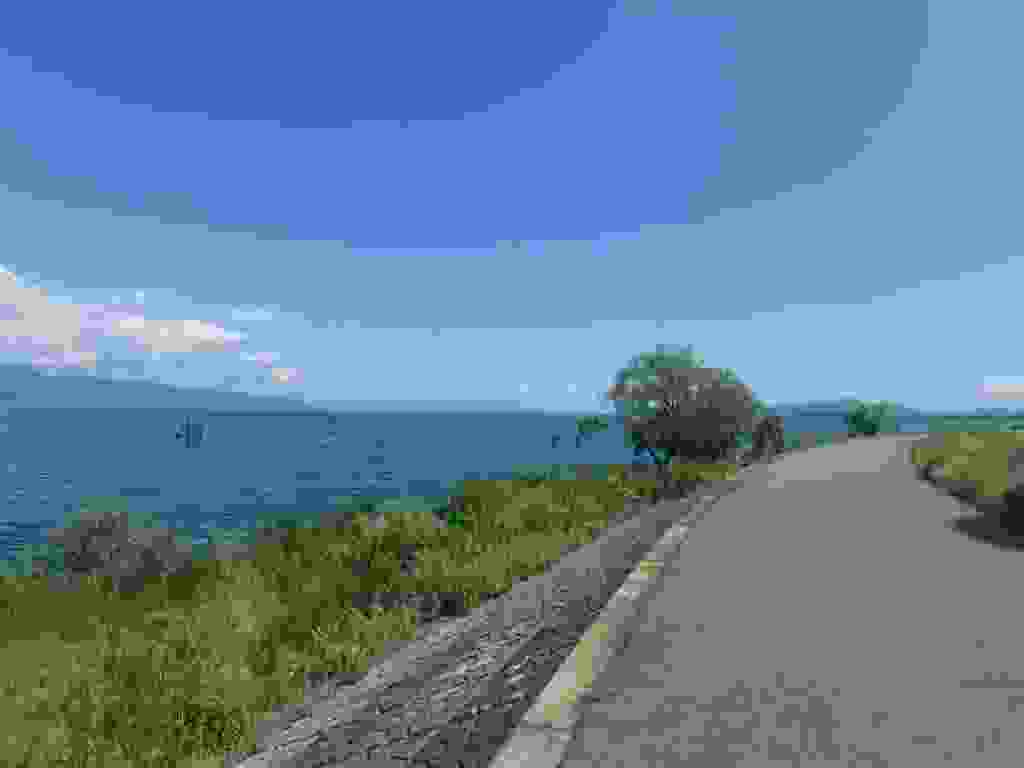
\includegraphics[width=\mywidth]{../wp-content/uploads/2015/08/P8186228-1024x768.jpg} \end{center}
\begin{center} 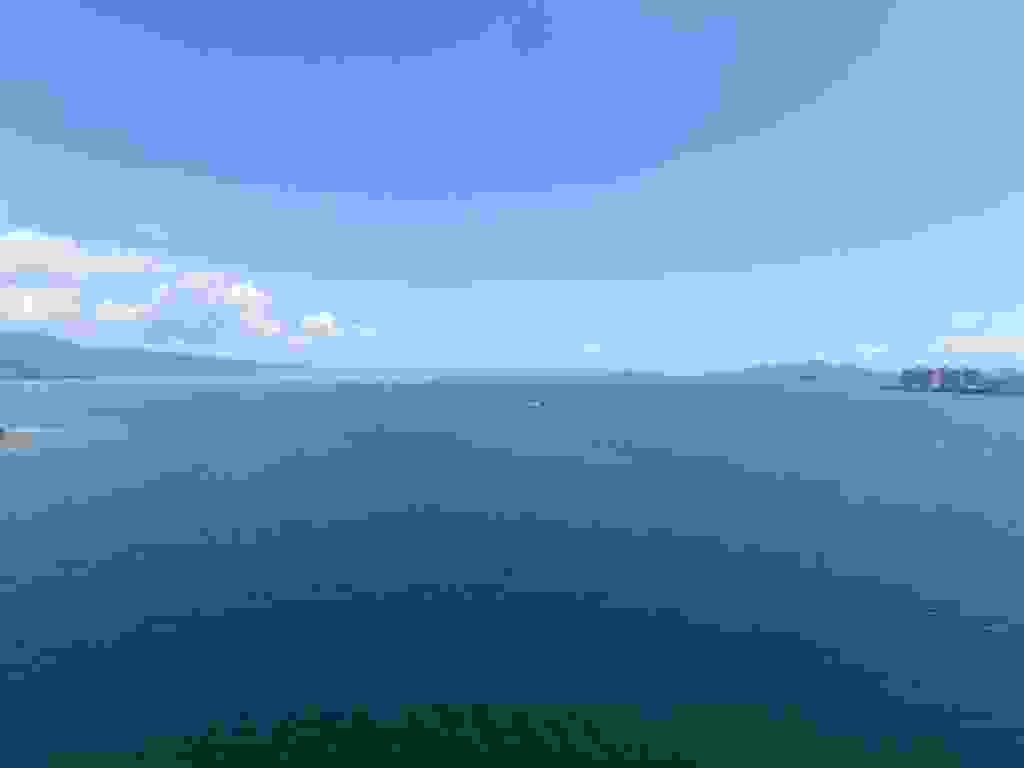
\includegraphics[width=\mywidth]{../wp-content/uploads/2015/08/P8186229-1024x768.jpg} \end{center}

 Quelques km avant Kyoto, arrêt pour visiter 2 temples.
\begin{center} 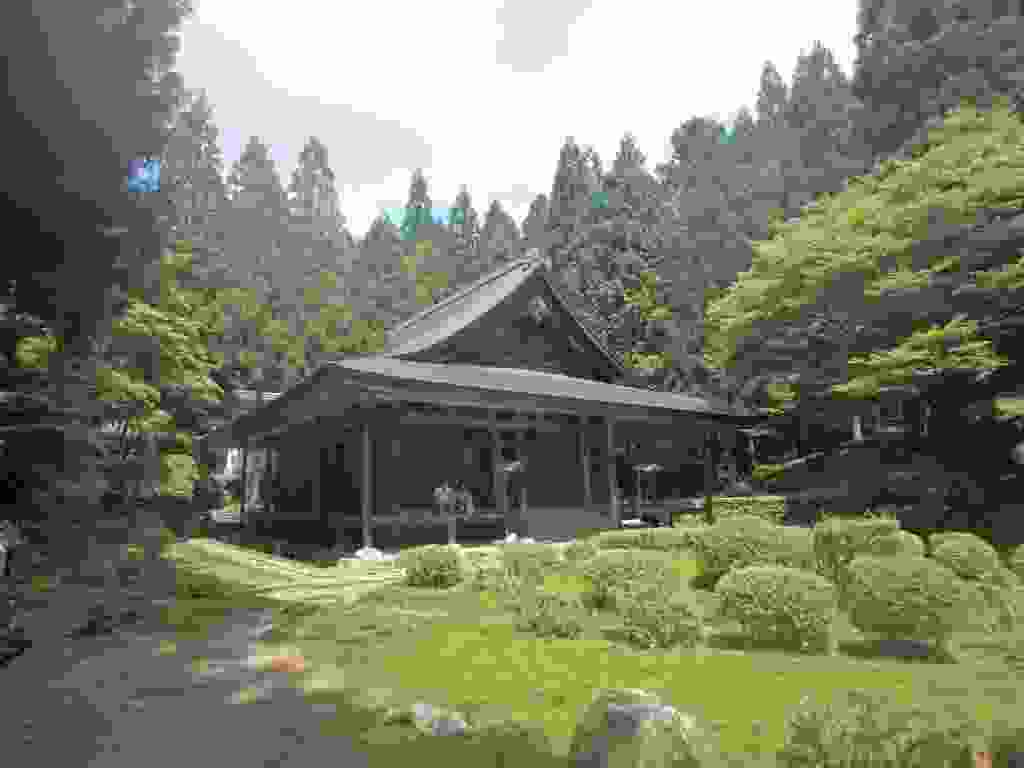
\includegraphics[width=\mywidth]{../wp-content/uploads/2015/08/P8186232-1024x768.jpg} \end{center}
\begin{center} 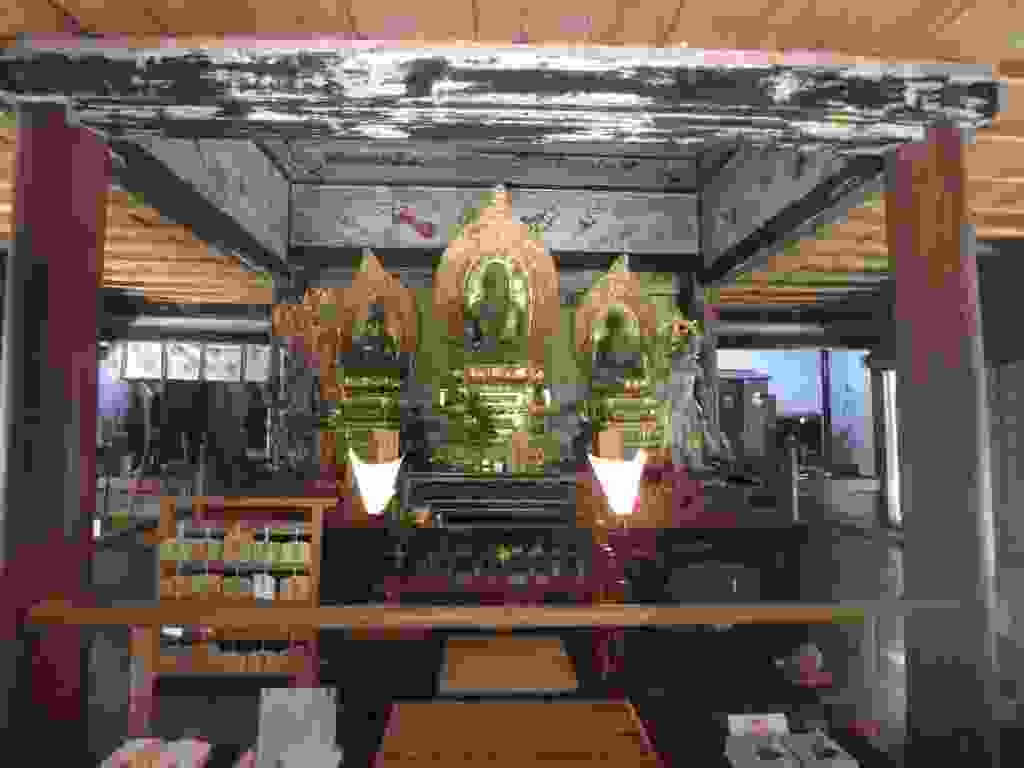
\includegraphics[width=\mywidth]{../wp-content/uploads/2015/08/P8186233-1024x768.jpg} \end{center}
\begin{center} 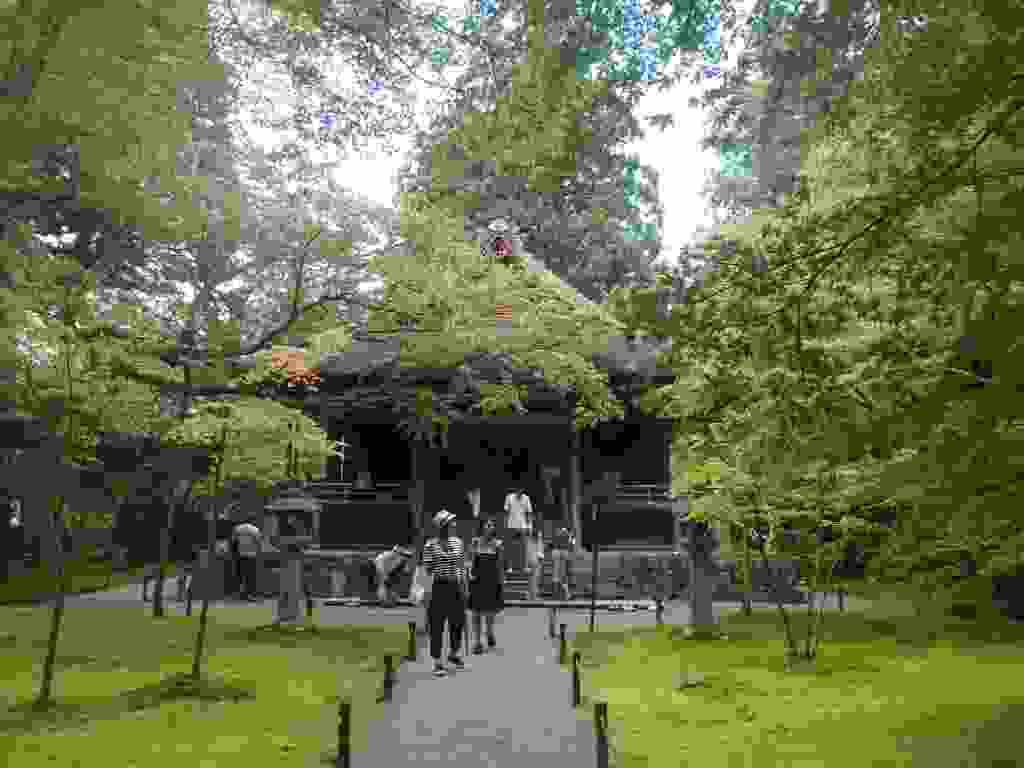
\includegraphics[width=\mywidth]{../wp-content/uploads/2015/08/P8186243-1024x768.jpg} \end{center}
\begin{center} 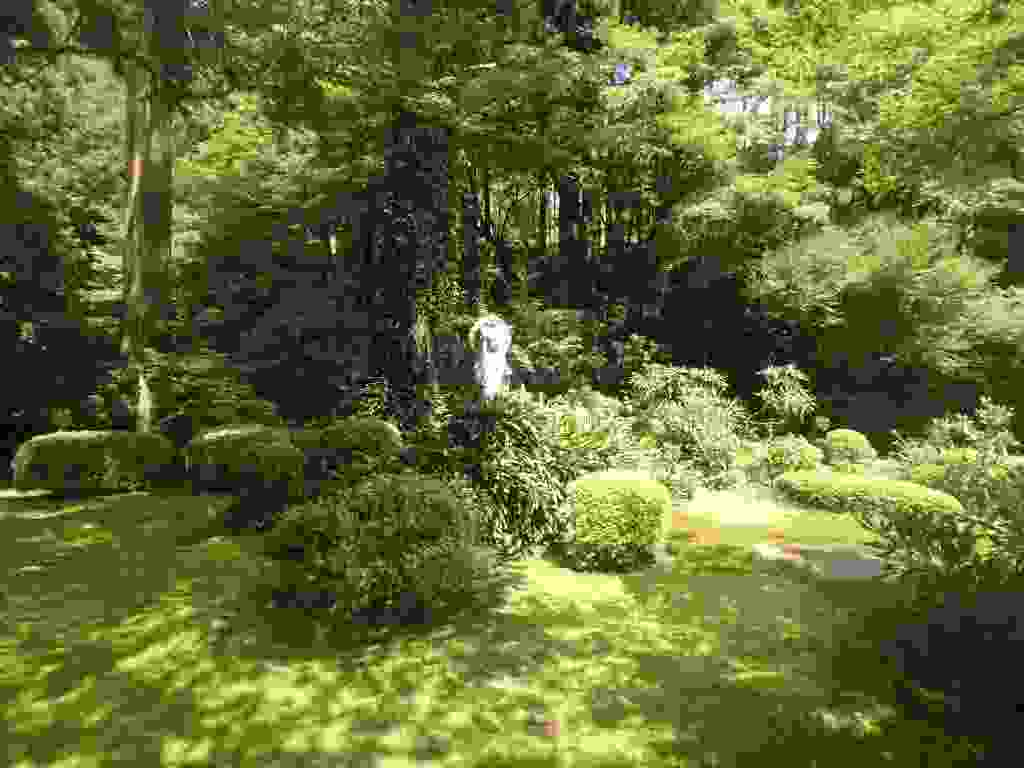
\includegraphics[width=\mywidth]{../wp-content/uploads/2015/08/P8186241-1024x768.jpg} \end{center}

 \`A Kyoto je suis recu par Ken qui est malaisien. 

 Il m'emmène goûter un okonomiyaki, galette à base de chou complétée par viande, fromage ou \oe{}uf selon les versions. 
\begin{center} 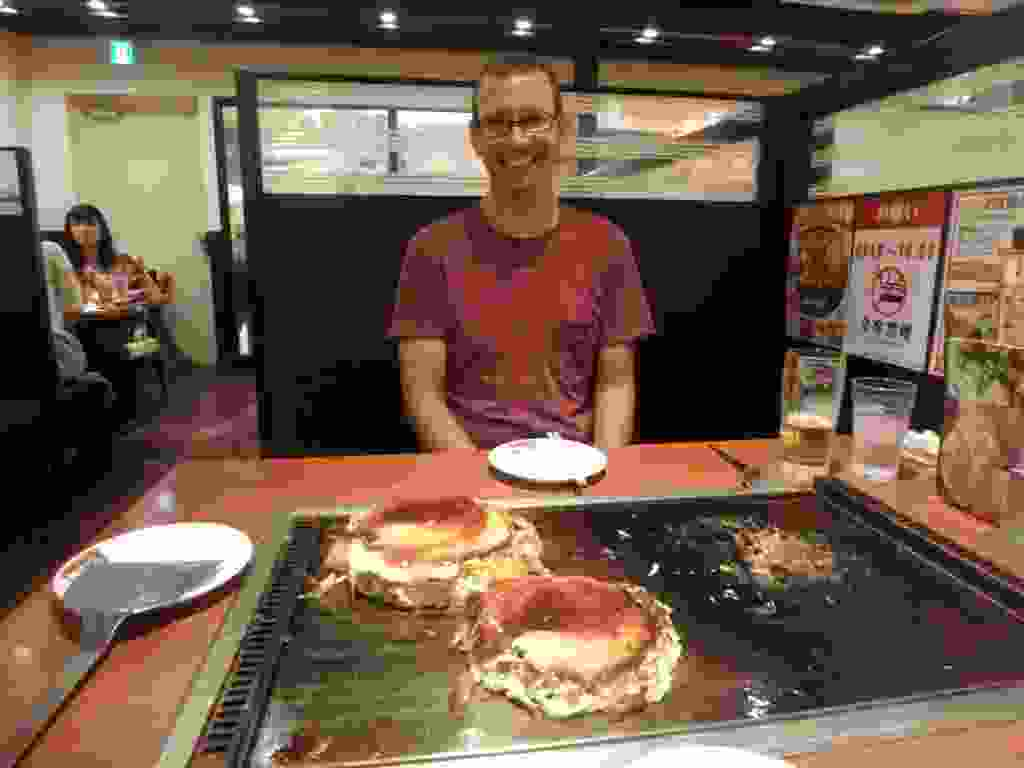
\includegraphics[width=\mywidth]{../wp-content/uploads/2015/08/P8196331-1024x768.jpg} \end{center}

\pagebreak
 Grâce à lui je rencontre Bruce et Chiara, un couple de cyclistes américains en vélos pliants. 
\begin{center} 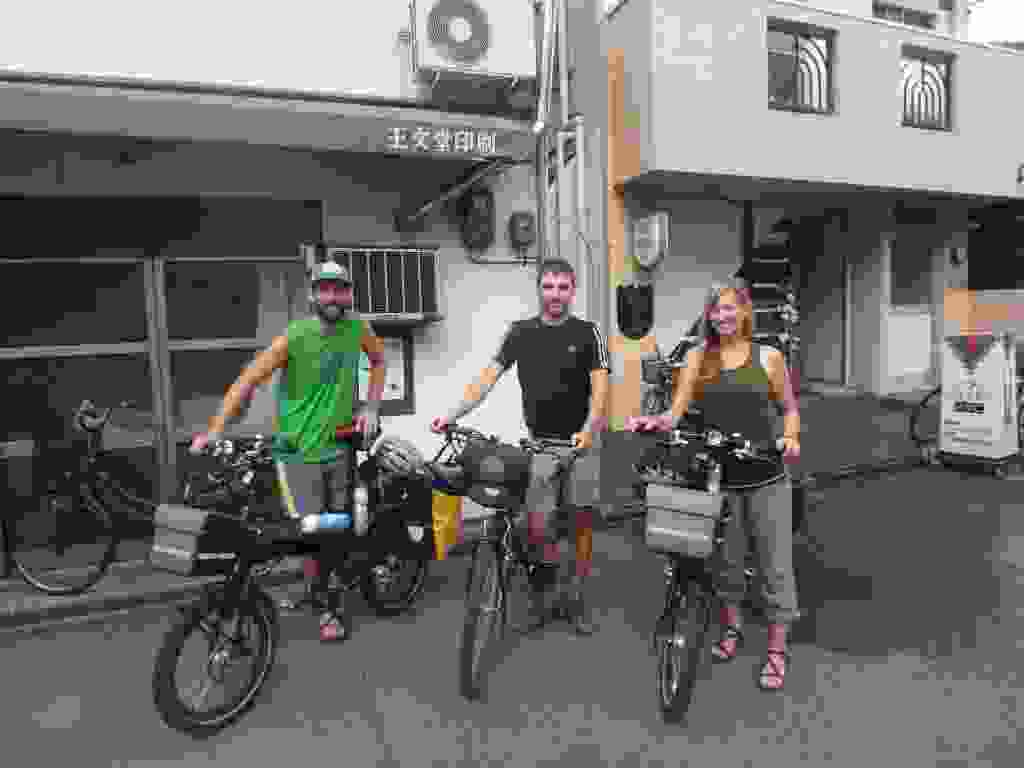
\includegraphics[width=\mywidth]{../wp-content/uploads/2015/08/P8196253-1024x768.jpg} \end{center}

 Il y a des centaines de temples et shrines à Kyoto, je suis allé en voir quelques-uns. 

 Shrine Fushimi Inari-taisha et ses milliers de portes.
\begin{center} 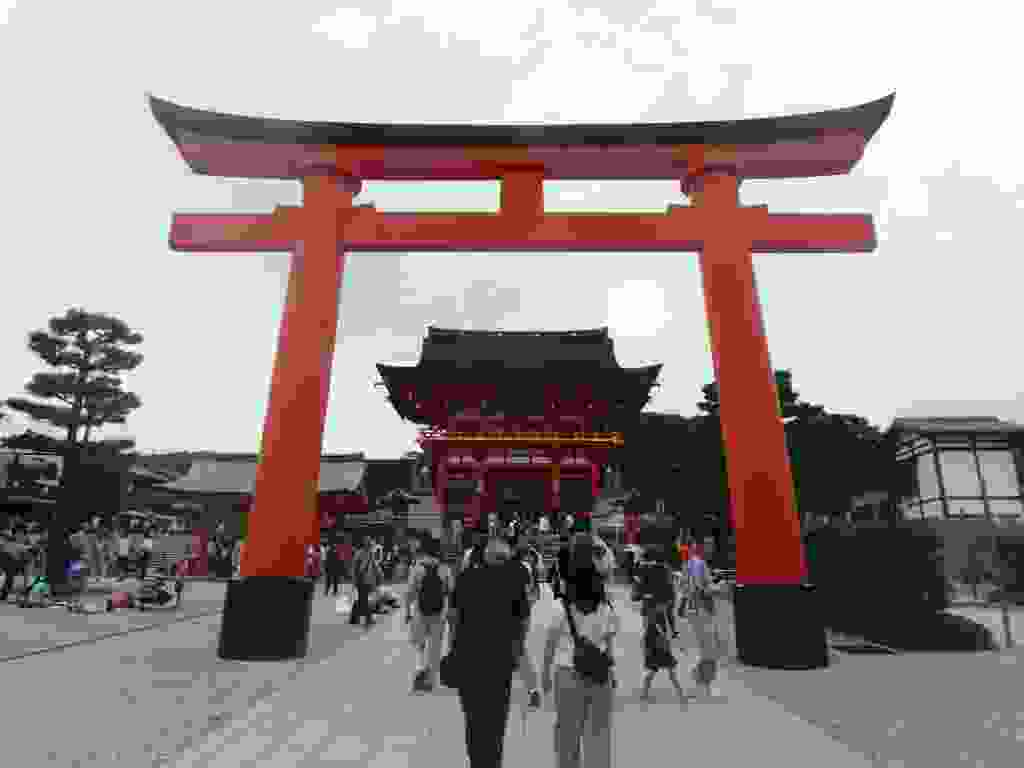
\includegraphics[width=\mywidth]{../wp-content/uploads/2015/08/P8196254-1024x768.jpg} \end{center}
\begin{center} 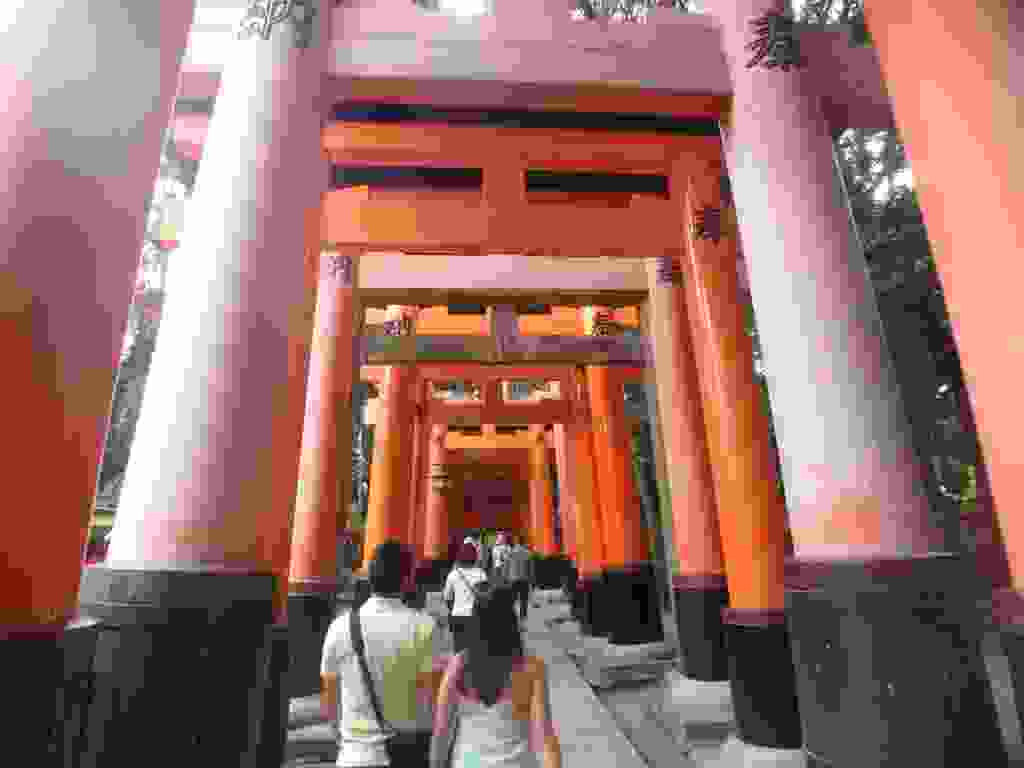
\includegraphics[width=\mywidth]{../wp-content/uploads/2015/08/P8196257-1024x768.jpg} \end{center}
\begin{center} 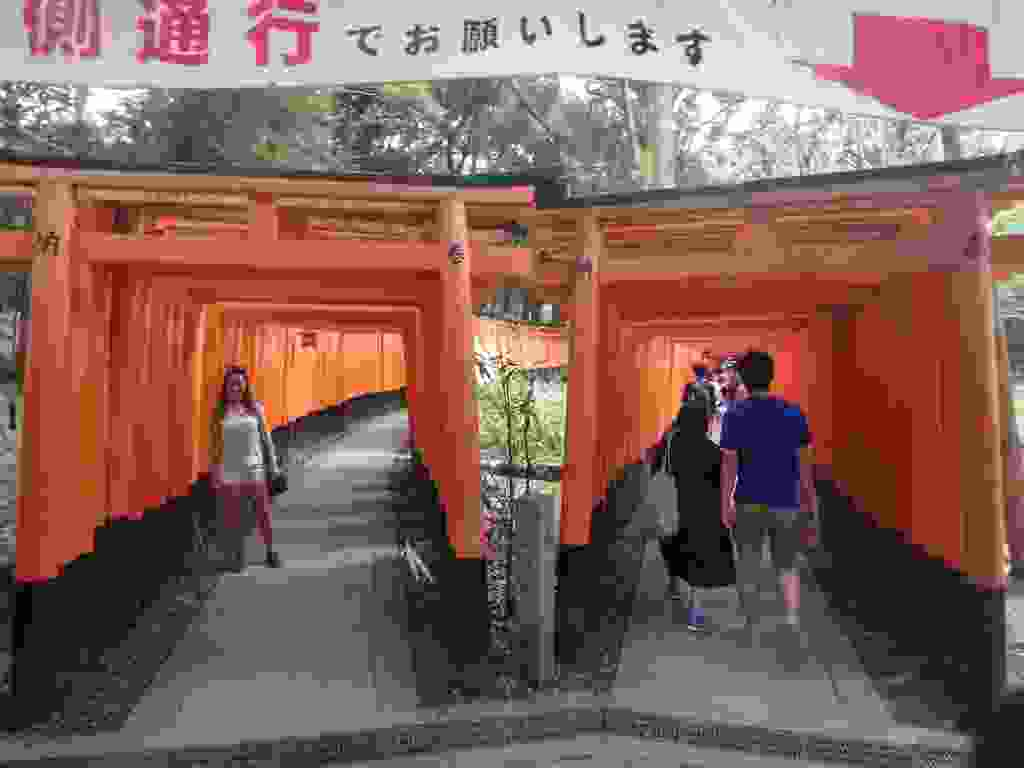
\includegraphics[width=\mywidth]{../wp-content/uploads/2015/08/P8196259-1024x768.jpg} \end{center}

\pagebreak
 Shrine Shimogamo, un des plus anciens du Japon.
\begin{center} 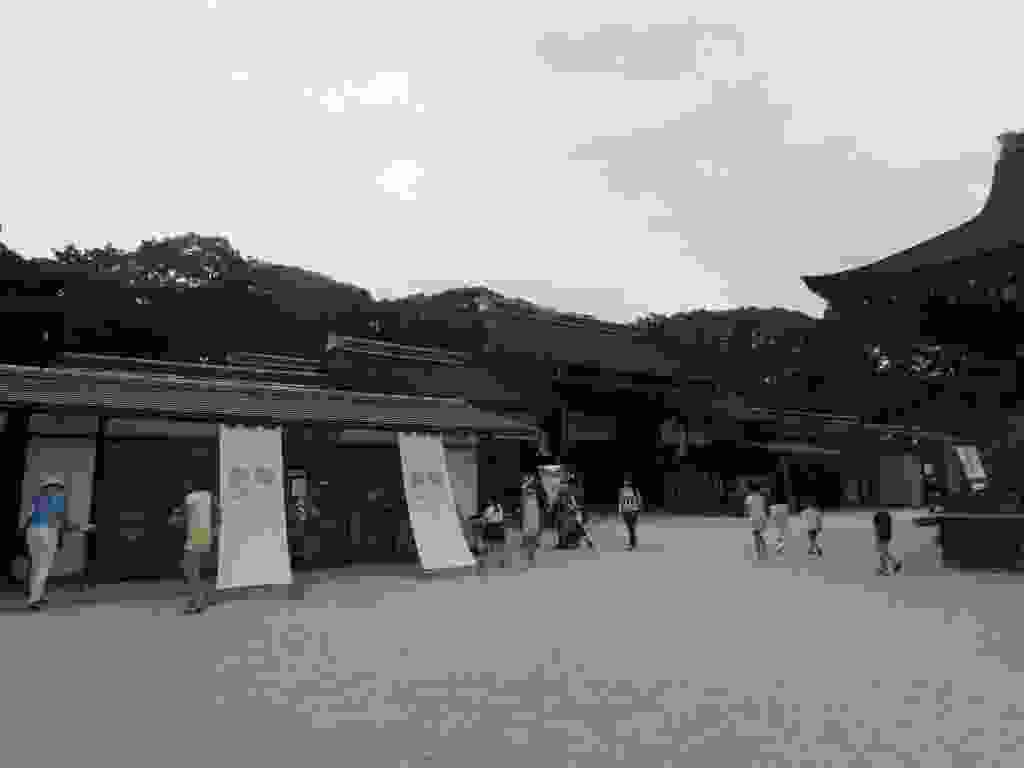
\includegraphics[width=\mywidth]{../wp-content/uploads/2015/08/P8196267-1024x768.jpg} \end{center}

 Ginkaku-ji, le pavillon d'argent.
\begin{center} 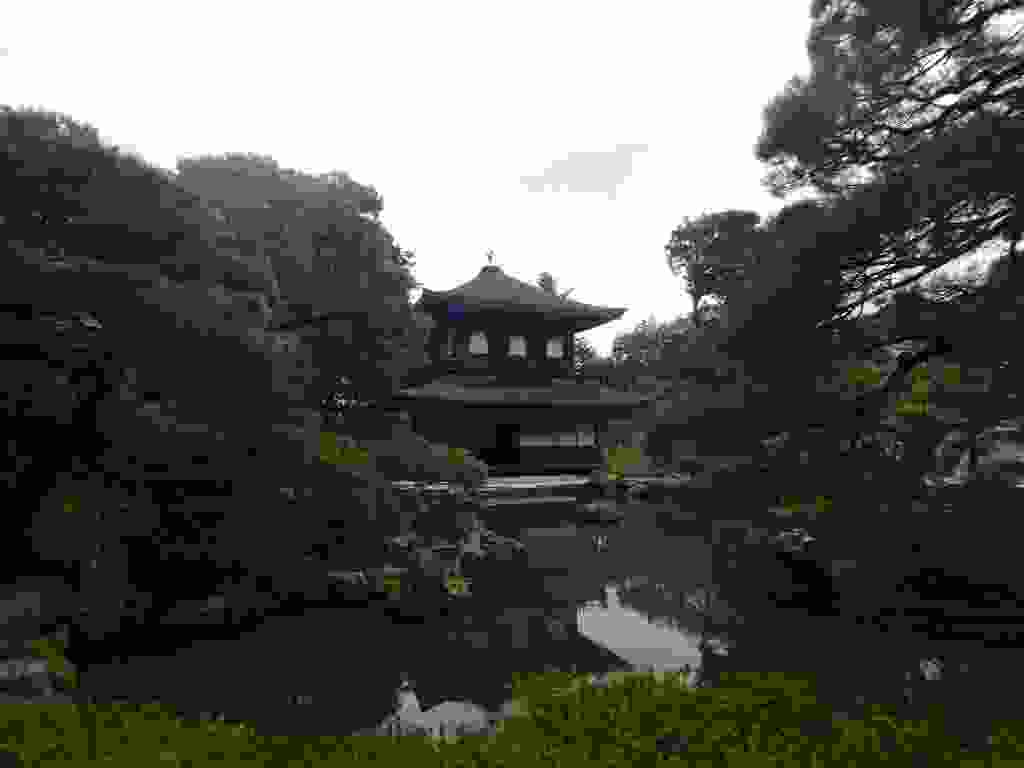
\includegraphics[width=\mywidth]{../wp-content/uploads/2015/08/P8196284-1024x768.jpg} \end{center}
\begin{center} 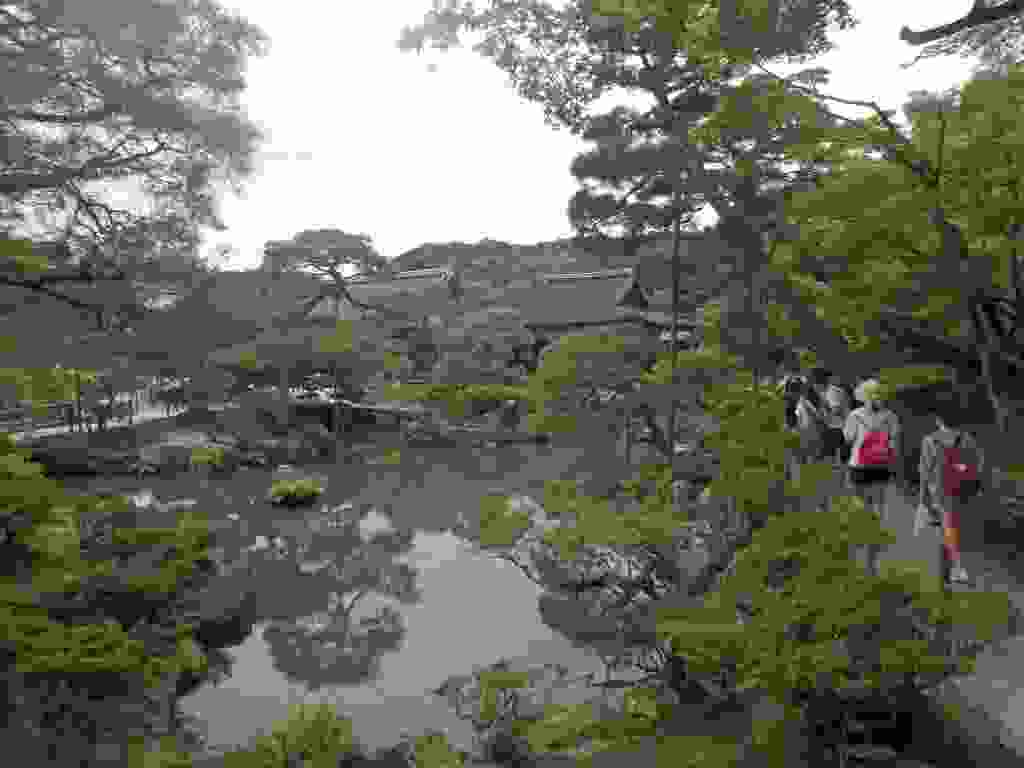
\includegraphics[width=\mywidth]{../wp-content/uploads/2015/08/P8196278-1024x768.jpg} \end{center}

 Temple Kiyomizu-dera, peut-être le plus visité de Kyoto.
\begin{center} 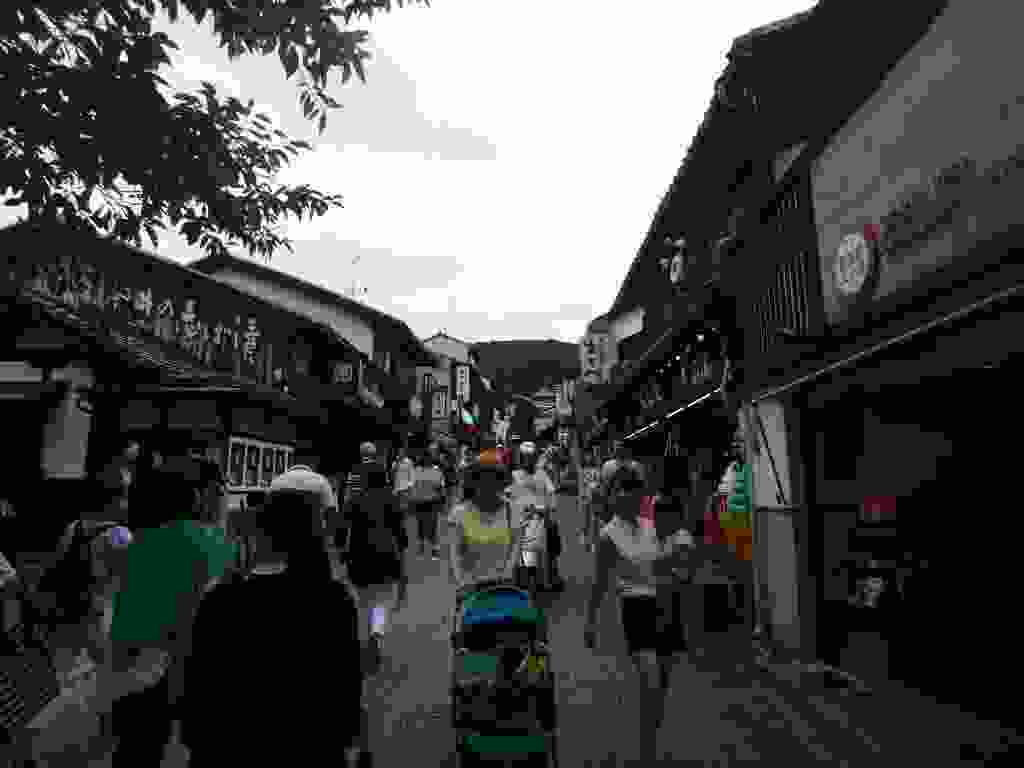
\includegraphics[width=\mywidth]{../wp-content/uploads/2015/08/P8196296-1024x768.jpg} \end{center}
\begin{center} 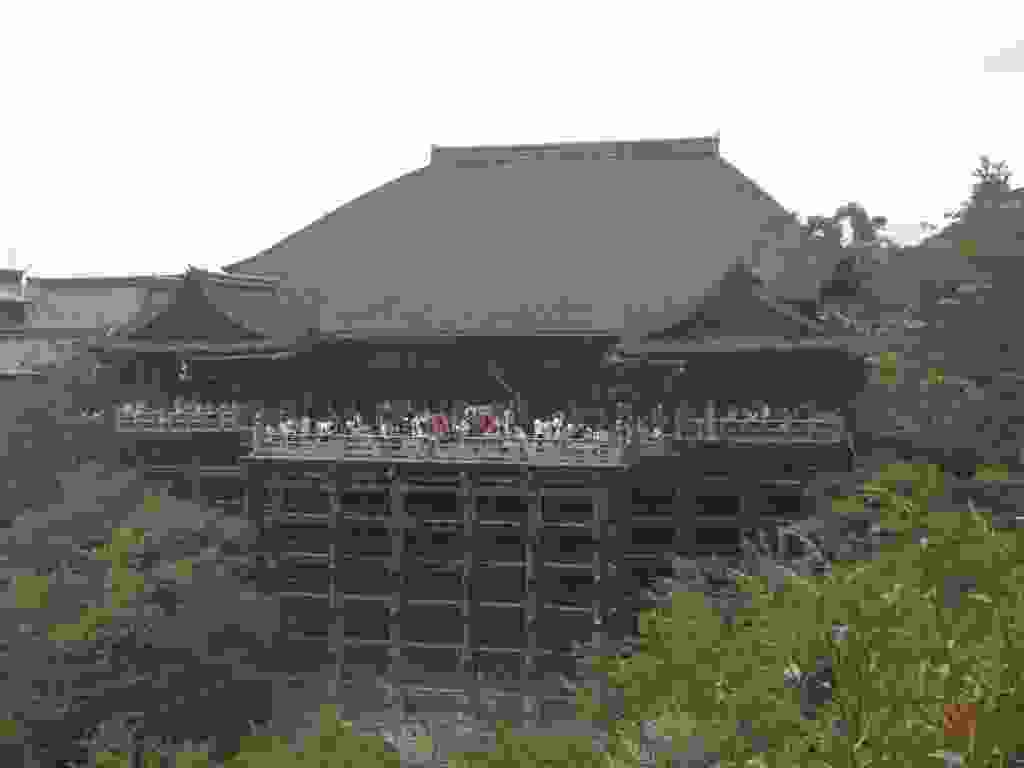
\includegraphics[width=\mywidth]{../wp-content/uploads/2015/08/P8196308-1024x768.jpg} \end{center}

 Temple Nishi Hongan-ji, le seul de ceux que j'ai vu qui n'était pas seulement touristique, avec des moines dedans.
\begin{center} 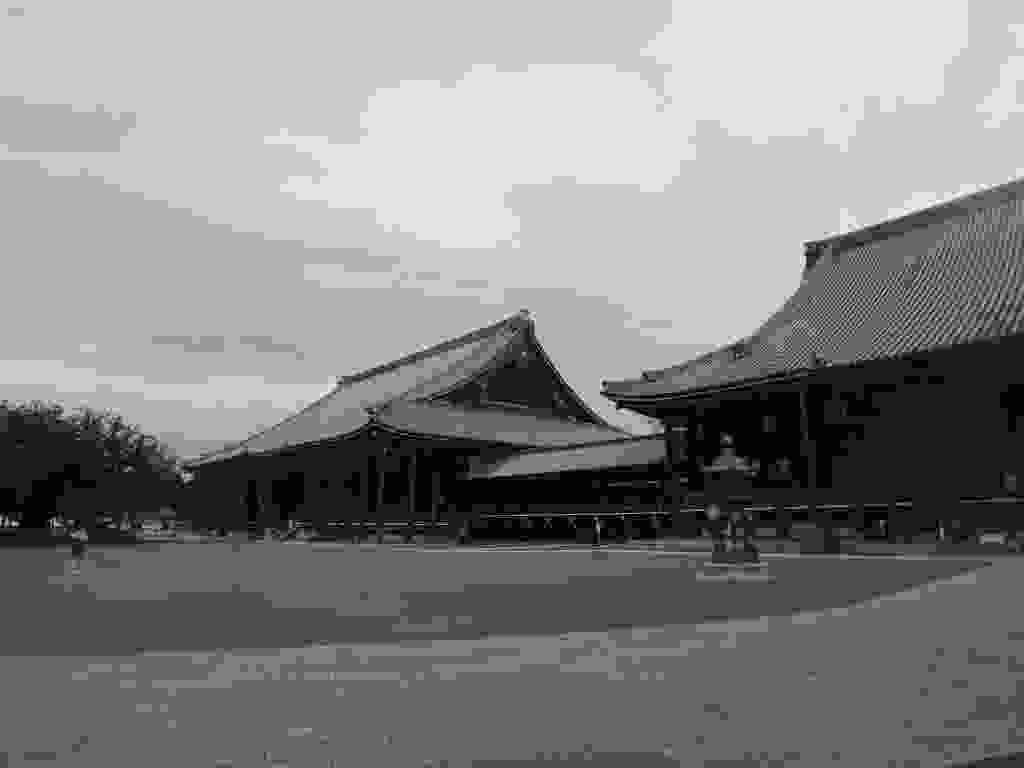
\includegraphics[width=\mywidth]{../wp-content/uploads/2015/08/P8196320-1024x768.jpg} \end{center}
\begin{center} 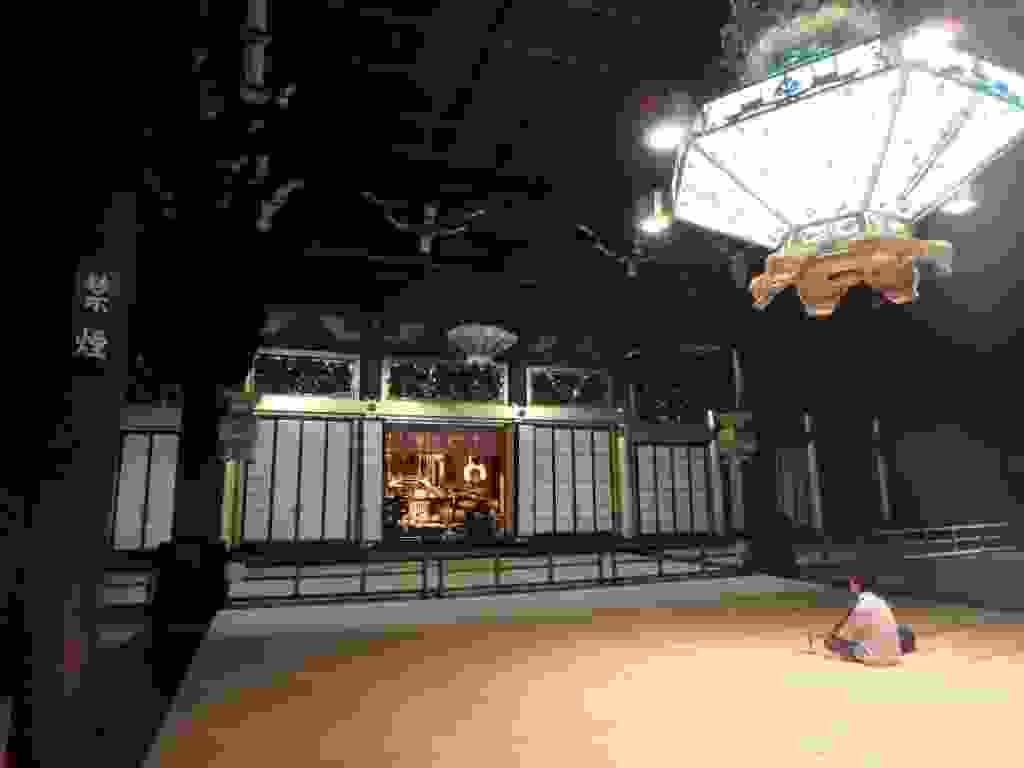
\includegraphics[width=\mywidth]{../wp-content/uploads/2015/08/P8196322-1024x768.jpg} \end{center}

 Le vieux quartier de Gion.
\begin{center} 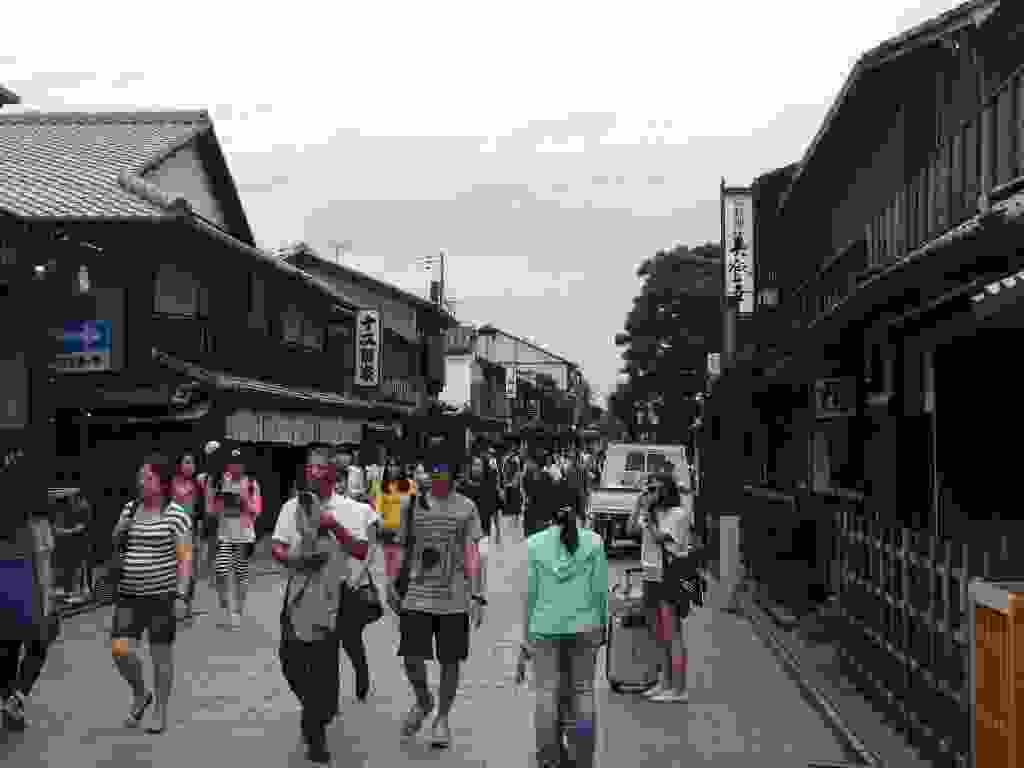
\includegraphics[width=\mywidth]{../wp-content/uploads/2015/08/P8196314-1024x768.jpg} \end{center}

\pagebreak
 Kyoto Station, un peu de modernité.
\begin{center} 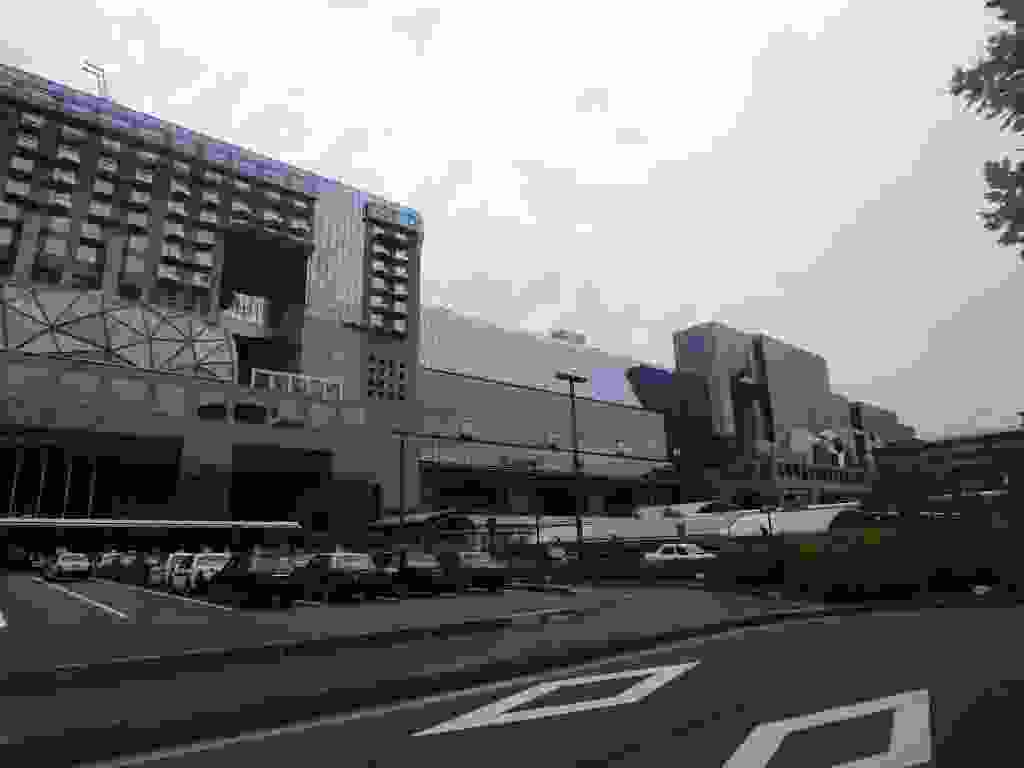
\includegraphics[width=\mywidth]{../wp-content/uploads/2015/08/P8196315-1024x768.jpg} \end{center}

 Parking à vélo dans un centre commercial.
\begin{center} 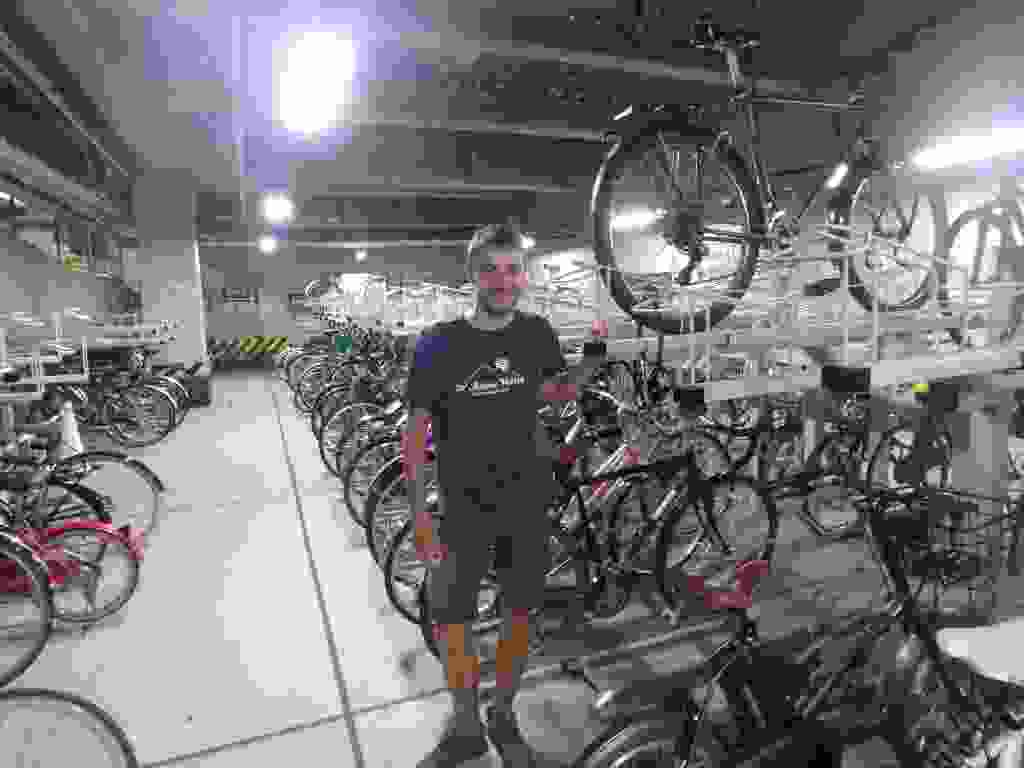
\includegraphics[width=\mywidth]{../wp-content/uploads/2015/08/P8196327-1024x768.jpg} \end{center}

\pagebreak
 Un immense magasin de produits électroniques, finalement c'est tout petit la fnac. 
\begin{center} 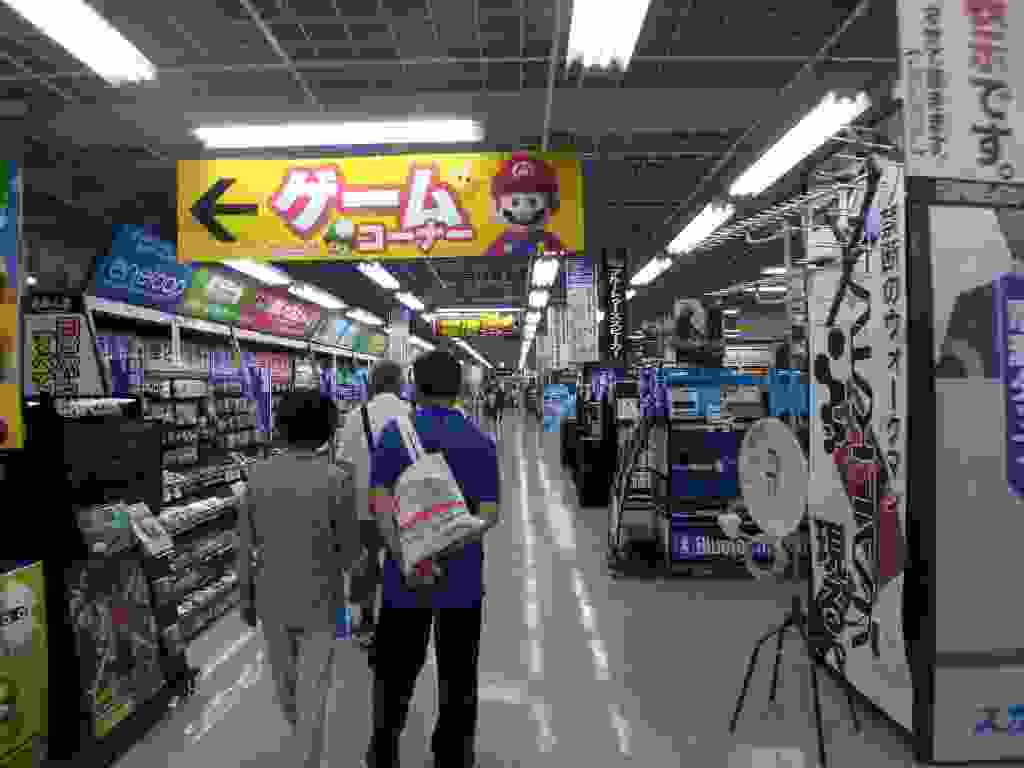
\includegraphics[width=\mywidth]{../wp-content/uploads/2015/08/P8196329-1024x768.jpg} \end{center}
